\section{Configuración experimental}

\subsection{Datos de entrenamiento}


Para nuestros modelos por defecto, entrenamos el modelo sobre 370K videos de instruction tuning agregados a partir de una colección de datasets, incluidos YouCook2~\cite{zhou2018youcook2}, Ego4D-HCap~\cite{islam2024video}, NExT-QA~\cite{xiao2021nextqa}, IntentQA~\cite{li2023intentqa}, CLEVRER~\cite{yi2020clevrer}, Ego4D~\cite{Grauman2021Ego4DAT}, STAR~\cite{wu2024star} y Perception Test~\cite{patraucean2023perception}. No utilizamos ningún dato generado por ChatGPT o GPT-4, de acuerdo con los términos de uso de OpenAI\footnote{\href{https://openai.com/policies/row-terms-of-use}{https://openai.com/policies/row-terms-of-use}} y nuestra política legal interna. Además, para acelerar los experimentos de ablation, construimos un conjunto de entrenamiento de instruction tuning más pequeño de 70K videos a partir de NExT-QA~\cite{xiao2021nextqa}, IntentQA~\cite{li2023intentqa}, Ego4D~\cite{Grauman2021Ego4DAT} y Ego4D-HCap~\cite{islam2024video}. Las ablaciones se evalúan en NExT-QA~\cite{xiao2021nextqa} y EgoSchema~\cite{mangalam2023egoschema}.


\subsection{Benchmarks de evaluación}
Evaluamos nuestro modelo en siete benchmarks diversos de video question-answering: Perception Test~\cite{patraucean2024perception}, NExT-QA~\cite{xiao2021nextqa}, EgoSchema~\cite{mangalam2023egoschema}, VNBench~\cite{zhao2024needle}, LongVideoBench~\cite{wu2024longvideobench}, Video-MME~\citep{fu2024video} y MLVU~\cite{zhou2024mlvu}. 

\subsection{Variantes de nuestro modelo}
\begin{itemize}

\item \textbf{\modelLlava.} Implementamos esta variante aplicando \model\ sobre el image-pretrained MLLM LLaVA-NeXT~\cite{liu2024llavanext}, que utiliza el vision encoder CLIP~\cite{radford2021learning} y el LLM Vicuna-7B~\cite{vicuna2023}.  

\item \textbf{\modelLlama.} Implementamos esta variante aplicando \model\ sobre el image-pretrained MLLM LLaMA-3.2~\cite{llama3.2}, que utiliza el vision encoder Meta-CLIP~\cite{xu2023demystifying} y el LLM LLaMA-3.2-LLM-8B.

\end{itemize}

\subsection{Baselines}

Además de comparar con métodos previos basados en distintos MLLMs y entrenados con datos diferentes, implementamos los siguientes baselines para una comparación justa.

\begin{itemize}

\item \textbf{Vanilla.} Implementamos este baseline eliminando el spatiotemporal token selector de nuestro modelo, lo que da como resultado ausencia de compresión de tokens. Todos los tokens generados por el image encoder se pasan directamente al LLM.

\item \textbf{Pooling.} Este baseline aplica spatiotemporal pooling como método de compresión, utilizando la misma razón de compresión que nuestro modelo principal. 

\item \textbf{Self-Attention.} Implementamos este baseline reemplazando la capa selective-scan de nuestro spatiotemporal token selector por capas self-attention. 

\item \textbf{Perceiver.} Este baseline aprovecha el mecanismo Perceiver~\cite{jaegle2021perceiver} para comprimir tokens espaciotemporales y usa la misma razón de compresión que nuestro modelo.

\end{itemize}

\begin{figure*}[t]
\footnotesize
\centering
\vspace{-10mm}
\captionsetup[subfigure]{margin={-20mm,-5mm}}
\begin{subfigure}[b]{0.48\textwidth}
    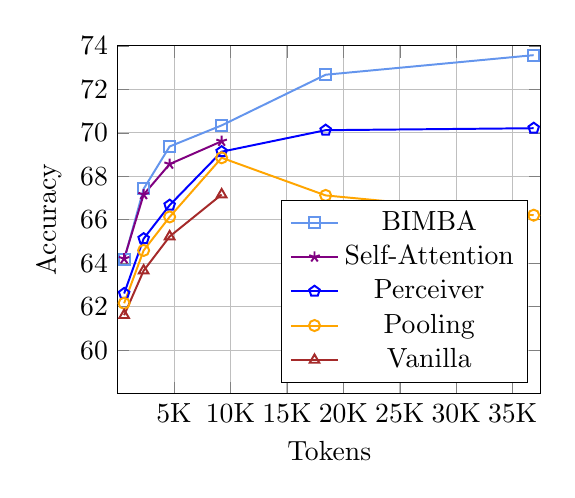
\begin{tikzpicture}
    \begin{axis}[
        % width=12cm, 
        height=6cm,
        xlabel={Tokens},
        ylabel={Accuracy},
        %title={(a) LLaVA Backbone on NeXT-QA},
        xmin=0, xmax=37500,
        ymin=58, ymax=74,
        %xtick={576, 2304, 4608, 9216, 18432, 36864},
        % xticklabels={576, 2304, 4608, 9216, 18432, 36864},
        xtick={5000, 10000, 15000, 20000,25000,30000, 35000},
        xticklabels={5K, 10K, 15K, 20K, 25K,30K, 35K},
        ytick={60, 62, 64, 66, 68, 70, 72, 74},
        legend pos=south east,
        grid=both,
        scaled ticks = false,
        scaled x ticks = false,
        % xmode=log,
        % log basis x=1
    ]
    % BIMBA Data
    \addplot[line width=.25mm, color=CornflowerBlue, mark=square, mark size=2pt]
    coordinates {
    (576, 64.16) (2304, 67.42) (4608, 69.37) (9216, 70.34) (18432, 72.67) (36864, 73.57)
    };
    \addlegendentry{BIMBA}
    
    % Self-Attention Data
    \addplot[line width=.25mm, color=Purple, mark=star, mark size=2pt]
        coordinates {
        (576, 64.21) (2304, 67.16) (4608, 68.56) (9216, 69.61)
    };
    \addlegendentry{Self-Attention}

    \addplot[line width=.25mm, color=Blue, mark=pentagon, mark size=2pt]
    coordinates {
    (576, 62.61) (2304, 65.13) (4608, 66.67) (9216, 69.13) (18432, 70.12) (36864, 70.21)
    };
    \addlegendentry{Perceiver}
    
    % Pooling Data
    \addplot[line width=.25mm, color=Orange, mark=o, mark size=2pt]
    coordinates {
    (576, 62.16) (2304, 64.59) (4608, 66.13) (9216, 68.85) (18432, 67.12) (36864, 66.21)
    };
    \addlegendentry{Pooling}

    \addplot[line width=.25mm, color=Brown, mark=triangle, mark size=2pt]
    coordinates {
    (576, 61.61) (2304, 63.66) (4608, 65.23) (9216, 67.16) 
    };
    \addlegendentry{Vanilla}
    \end{axis}
    \end{tikzpicture}
    \vspace{-1mm}
    \caption{NExT-QA performance of models based on LLaVA.}
    \vspace{1mm}
\end{subfigure}
\hfill
\begin{subfigure}[b]{0.48\textwidth}
    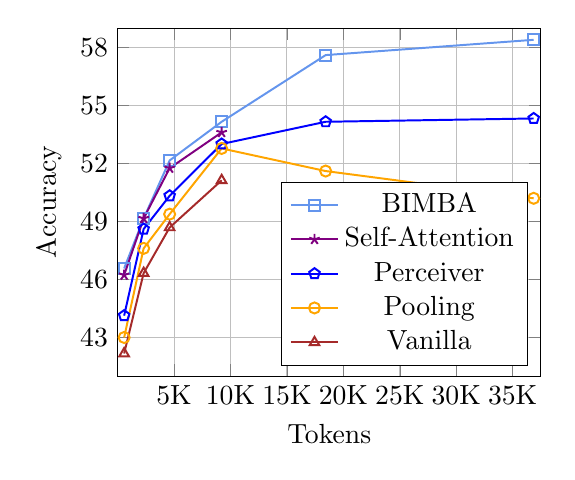
\begin{tikzpicture}
    \begin{axis}[
        % width=12cm, height=8cm,
        %height=7cm,
        height=6cm,
        xlabel={Tokens},
        ylabel={Accuracy},
        %title={(b) LLaVA Backbone on EgoSchema},
        xmin=0, xmax=37500,
        ymin=41, ymax=59,
        %xtick={576, 2304, 4608, 9216, 18432, 36864},
        % xticklabels={576, 2304, 4608, 9216, 18432, 36864},
        xtick={5000, 10000, 15000, 20000,25000,30000, 35000},
        xticklabels={5K, 10K, 15K, 20K, 25K,30K, 35K},
        ytick={43, 46, 49, 52, 55, 58, 61},
        legend pos=south east,
        grid=both,
        scaled ticks = false,
        scaled x ticks = false,
        % xmode=log,
        % log basis x=1
    ]
    % BIMBA Data
    \addplot[line width=.25mm, color=CornflowerBlue, mark=square, mark size=2pt]
    coordinates {
    (576, 46.57) (2304, 49.16) (4608, 52.16) (9216, 54.16) (18432, 57.61) (36864, 58.40)
    };
    \addlegendentry{BIMBA}

    % Self-Attention Data
    \addplot[line width=.25mm, color=Purple, mark=star, mark size=2pt]
        coordinates {
        (576, 46.23) (2304, 49.16) (4608, 51.76) (9216, 53.61)
    };
    \addlegendentry{Self-Attention}

    \addplot[line width=.25mm, color=Blue, mark=pentagon, mark size=2pt]
    coordinates {
    (576, 44.13) (2304, 48.61) (4608, 50.33) (9216, 53.01) (18432, 54.16) (36864, 54.33)
    };
    \addlegendentry{Perceiver}

    % Pooling Data
    \addplot[line width=.25mm, color=Orange, mark=o, mark size=2pt]
    coordinates {
    (576, 43.00) (2304, 47.61) (4608, 49.38) (9216, 52.78) (18432, 51.61) (36864, 50.20)
    };
    \addlegendentry{Pooling}

    \addplot[line width=.25mm, color=Brown, mark=triangle, mark size=2pt]
    coordinates {
    (576, 42.17) (2304, 46.33) (4608, 48.69) (9216, 51.13) 
    };
    \addlegendentry{Vanilla}
    \end{axis}
    \end{tikzpicture}
    \vspace{-1mm}
    \caption{EgoSchema performance of models based on LLaVA.}
    \vspace{1mm}
\end{subfigure}
\begin{subfigure}[b]{0.48\textwidth}
    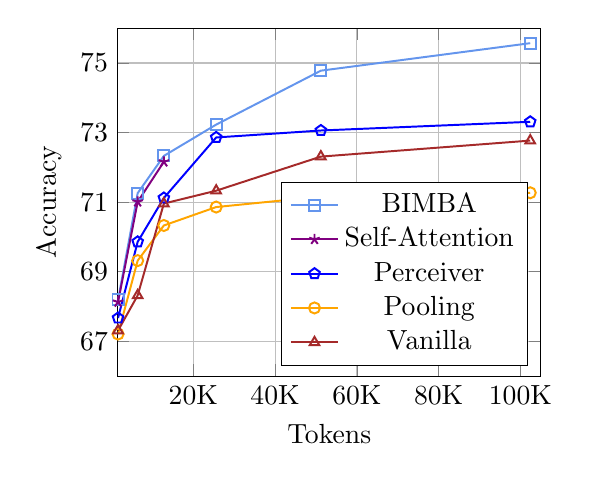
\begin{tikzpicture}
    \begin{axis}[
        % width=12cm, height=8cm,
        %height=7cm,
        height=6cm,
        xlabel={Tokens},
        ylabel={Accuracy},
        %title={(a) LLaMA Backbone on NeXT-QA},
        xmin=1500, xmax=105000,
        ymin=66, ymax=76,
        %xtick={1600, 6400, 12800, 25600, 51200, 102400},
        % xticklabels={1600, 6400, 12800, 25600, 51200, 102400},
        xtick={20000,40000,60000,80000,100000},
        xticklabels={20K, 40K, 60K, 80K, 100K},
        ytick={67, 69, 71, 73, 75, 77},
        legend pos=south east,
        grid=both,
        scaled ticks = false,
        scaled x ticks = false,
        % xmode=log,
        % log basis x=1
    ]
    % BIMBA Data
    \addplot[line width=.25mm, color=CornflowerBlue, mark=square, mark size=2pt]
    coordinates {
    (1600, 68.19) (6400, 71.26) (12800, 72.33) (25600, 73.23) (51200, 74.78) (102400, 75.57)
    };
    \addlegendentry{BIMBA}
    
    % Self-Attention Data
    \addplot[line width=.25mm, color=Purple, mark=star, mark size=2pt]
        coordinates {
        (1600, 68.13) (6400, 71.01) (12800, 72.16) 
    };
    \addlegendentry{Self-Attention}

    \addplot[line width=.25mm, color=Blue, mark=pentagon, mark size=2pt]
    coordinates {
    (1600, 67.67) (6400, 69.86) (12800, 71.12) (25600, 72.86) (51200, 73.06) (102400, 73.31)
    };
    \addlegendentry{Perceiver}
    
    % Pooling Data
    \addplot[line width=.25mm, color=Orange, mark=o, mark size=2pt]
    coordinates {
    (1600, 67.21) (6400, 69.32) (12800, 70.33) (25600, 70.86) (51200, 71.16) (102400, 71.27)
    };
    \addlegendentry{Pooling}
    \addplot[line width=.25mm, color=Brown, mark=triangle, mark size=2pt]
    coordinates {
    (1600, 67.31) (6400, 68.32) (12800, 70.96) (25600, 71.33) (51200, 72.31) (102400, 72.77)
    };
    \addlegendentry{Vanilla}
    \end{axis}
    \end{tikzpicture}
    \caption{NExT-QA performance of models based on LLaMA.}
% \caption{Figure 1}
\end{subfigure}
\hfill
\begin{subfigure}[b]{0.48\textwidth}
    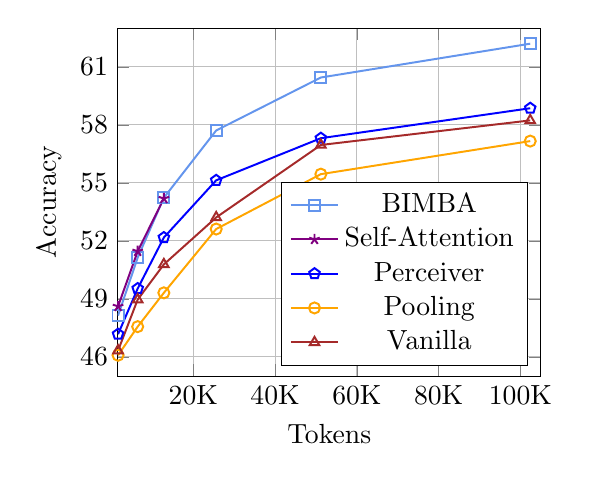
\begin{tikzpicture}
    \begin{axis}[
        % width=12cm, height=8cm,
        height=6cm,
        xlabel={Tokens},
        ylabel={Accuracy},
        %title={(b) LLaMA Backbone on EgoSchema},
        xmin=1500, xmax=105000,
        ymin=45, ymax=63,
        %xtick={1600, 6400, 12800, 25600, 51200, 102400},
        % xticklabels={1600, 6400, 12800, 25600, 51200, 102400},
        xtick={20000,40000,60000,80000,100000},
        xticklabels={20K, 40K, 60K, 80K, 100K},
        ytick={46, 49, 52, 55, 58, 61},
        legend pos=south east,
        grid=both,
        scaled ticks = false,
        scaled x ticks = false,
        % xmode=log,
        % log basis x=1
    ]
    % BIMBA Data
    \addplot[line width=.25mm, color=CornflowerBlue, mark=square, mark size=2pt]
    coordinates {
    (1600, 48.13) (6400, 51.13) (12800, 54.23) (25600, 57.71) (51200, 60.45) (102400, 62.20)
    };
    \addlegendentry{BIMBA}
    
    % Self-Attention Data
    \addplot[line width=.25mm, color=Purple, mark=star, mark size=2pt]
        coordinates {
        (1600, 48.61) (6400, 51.46) (12800, 54.19)
    };
    \addlegendentry{Self-Attention}

    \addplot[line width=.25mm, color=Blue, mark=pentagon, mark size=2pt]
    coordinates {
    (1600, 47.17) (6400, 49.53) (12800, 52.17) (25600, 55.13) (51200, 57.31) (102400, 58.86)
    };
    \addlegendentry{Perceiver}

    % Pooling Data
    \addplot[line width=.25mm, color=Orange, mark=o, mark size=2pt]
    coordinates {
    (1600, 46.08) (6400, 47.56) (12800, 49.31) (25600, 52.61) (51200, 55.45) (102400, 57.16)
    };
    \addlegendentry{Pooling}

    \addplot[line width=.25mm, color=Brown, mark=triangle, mark size=2pt]
    coordinates {
    (1600, 46.32) (6400, 48.96) (12800, 50.78) (25600, 53.21) (51200, 56.96) (102400, 58.23)
    };
    \addlegendentry{Vanilla}
    \end{axis}
    \end{tikzpicture}
    \caption{EgoSchema performance of models based on the LLaMA.}
\end{subfigure}
\vspace{-2mm}
\caption{\small{Accuracy achieved by \model\ and baseline models on NeXT-QA (left) and EgoSchema (right) as a function of the number of input tokens for models based on LLaVA (top row) and LLaMA (bottom row). \model\ achieves the highest accuracy for all sequence lengths, and the difference with other baselines increases as we 
increase the number of input tokens. Self-attention cannot be applied to long sequences as it causes GPU out-of-memory issues once the number of tokens becomes too large.}}
\vspace{-5mm}
\label{fig:performance1}
\end{figure*}

% \LT{add arrow and ``out of memory''}

\subsection{Detalles de implementación}

Usamos una estrategia simple para entrenar tanto nuestros modelos como los baselines: partiendo de un frame encoder image-pretrained, hacemos fine-tuning del MLLM sobre el dataset de video instruction-tuning. Congelamos el image encoder y entrenamos el spatiotemporal token selector y el LLM aplicando LoRA~\cite{hu2021lora} al LLM. Por defecto, el modelo \modelLlava toma 64 video frames divididos en $64 \times 24 \times 24 = 36,864$ tokens y comprime esta secuencia a $16 \times 12 \times 12 = 2,304$ tokens, que se pasan al LLM. Por defecto, \modelLlama procesa 64 frames divididos en $64 \times 40 \times 40 = 102,400$ tokens y comprime esta secuencia a $16 \times 20 \times 20 = 6,400$ tokens para el LLM.
